% Options for packages loaded elsewhere
\PassOptionsToPackage{unicode}{hyperref}
\PassOptionsToPackage{hyphens}{url}
\documentclass[
]{article}
\usepackage{xcolor}
\usepackage{amsmath,amssymb}
\setcounter{secnumdepth}{-\maxdimen} % remove section numbering
\usepackage{iftex}
\ifPDFTeX
  \usepackage[T1]{fontenc}
  \usepackage[utf8]{inputenc}
  \usepackage{textcomp} % provide euro and other symbols
\else % if luatex or xetex
  \usepackage{unicode-math} % this also loads fontspec
  \defaultfontfeatures{Scale=MatchLowercase}
  \defaultfontfeatures[\rmfamily]{Ligatures=TeX,Scale=1}
\fi
\usepackage{lmodern}
\ifPDFTeX\else
  % xetex/luatex font selection
\fi
% Use upquote if available, for straight quotes in verbatim environments
\IfFileExists{upquote.sty}{\usepackage{upquote}}{}
\IfFileExists{microtype.sty}{% use microtype if available
  \usepackage[]{microtype}
  \UseMicrotypeSet[protrusion]{basicmath} % disable protrusion for tt fonts
}{}
\makeatletter
\@ifundefined{KOMAClassName}{% if non-KOMA class
  \IfFileExists{parskip.sty}{%
    \usepackage{parskip}
  }{% else
    \setlength{\parindent}{0pt}
    \setlength{\parskip}{6pt plus 2pt minus 1pt}}
}{% if KOMA class
  \KOMAoptions{parskip=half}}
\makeatother
\usepackage{longtable,booktabs,array}
\newcounter{none} % for unnumbered tables
\usepackage{calc} % for calculating minipage widths
% Correct order of tables after \paragraph or \subparagraph
\usepackage{etoolbox}
\makeatletter
\patchcmd\longtable{\par}{\if@noskipsec\mbox{}\fi\par}{}{}
\makeatother
% Allow footnotes in longtable head/foot
\IfFileExists{footnotehyper.sty}{\usepackage{footnotehyper}}{\usepackage{footnote}}
\makesavenoteenv{longtable}
\usepackage{graphicx}
\makeatletter
\newsavebox\pandoc@box
\newcommand*\pandocbounded[1]{% scales image to fit in text height/width
  \sbox\pandoc@box{#1}%
  \Gscale@div\@tempa{\textheight}{\dimexpr\ht\pandoc@box+\dp\pandoc@box\relax}%
  \Gscale@div\@tempb{\linewidth}{\wd\pandoc@box}%
  \ifdim\@tempb\p@<\@tempa\p@\let\@tempa\@tempb\fi% select the smaller of both
  \ifdim\@tempa\p@<\p@\scalebox{\@tempa}{\usebox\pandoc@box}%
  \else\usebox{\pandoc@box}%
  \fi%
}
% Set default figure placement to htbp
\def\fps@figure{htbp}
\makeatother
\setlength{\emergencystretch}{3em} % prevent overfull lines
\providecommand{\tightlist}{%
  \setlength{\itemsep}{0pt}\setlength{\parskip}{0pt}}
\usepackage{bookmark}
\IfFileExists{xurl.sty}{\usepackage{xurl}}{} % add URL line breaks if available
\urlstyle{same}
\hypersetup{
  hidelinks,
  pdfcreator={LaTeX via pandoc}}

\author{}
\date{}

\begin{document}

Manufacturing and Assembly of a sub-scale prototype and full-scale
demonstrator of a Curved Canted Cosine Theta (CCCT) Dipole magnet

\section*{Abstract}

\textbf{This paper reports on the manufacturing and assembly of a
sub-scale prototype and a full-scale demonstrator of a curved Canted
Cosine Theta (CCCT) dipole magnet at CERN's main workshop. It outlines
the challenges associated with the fabrication of curved formers and the
solutions that were selected, including the nonconventional joining
technique and toolpath programming approach. The successful
manufacturing and assembly of both demonstrators confirm the feasibility
of curved CCT magnets and highlight their potential for future
accelerator applications and compact magnetic systems.}

Alan Saillet\textsuperscript{1}, Florian Hofmann \textsuperscript{1},
Jorge Guardia Valenzuela\textsuperscript{1}, Jean-Sébastien
Rigaud\textsuperscript{1}, Maciej Burkowski\textsuperscript{1}, Ariel
Haziot\textsuperscript{1}, Marco Garlasche\textsuperscript{1}, and Glyn
Kirby\textsuperscript{1}

\textsuperscript{1} CERN, Geneva, Switzerland

\section*{Introduction}

CCCT Magnets consist of two nested solenoids with opposed tilt angles
with the conductor placed in machined channels
(\hyperref[_Ref225570545]{Figure 1}, \hyperref[_Ref225751343]{Figure
2}). The shape and position of the channels determine the magnetic
properties and field homogeneity. In order to form a coil, conductors
are inserted in these grooved mandrels, called formers.

\begin{figure}
\centering
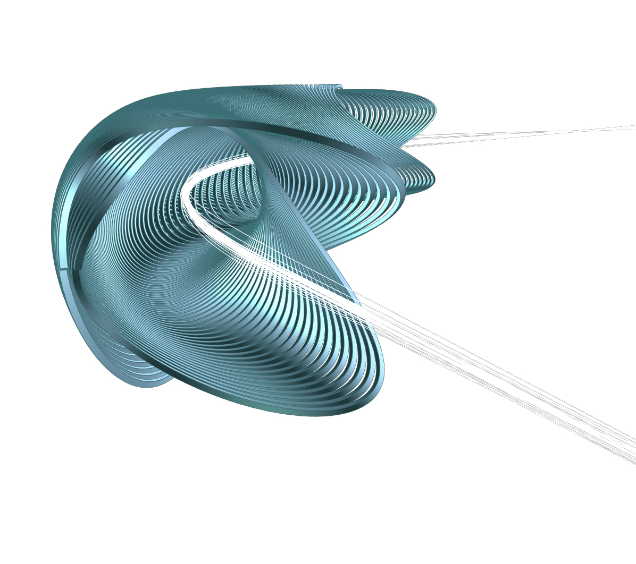
\includegraphics[width=2.83465in,height=1.80009in]{images/media/image1.png}
\caption{\protect\phantomsection\label{_Ref225570545}{}\textbf{Figure
1.} Simplified illustration of the CCCT concept, showing inner and outer
superconducting windings and the particle beam passing through the
aperture. (Image courtesy of TE-MSC-SMT)}
\end{figure}

This concept for a superconductive magnet has been introduced at CERN
for the Hi-Lumi orbit corrector MCBRD {[}1{]}. It has also attracted
attention as a promising design for compact accelerators and gantry
systems used in hadron therapy. This geometry offers considerable
flexibility in generating complex field harmonics in both straight and
curved configurations, where compactness is particularly advantageous.
The Fusillo Project has been proposed for the HIE-ISOLDE Recoil
Separator Ring {[}2{]}. The geometry of the full-scale demonstrator
forms a 90° bend with a curvature radius of 1 m and an aperture of 236
mm.

\begin{figure}
\centering
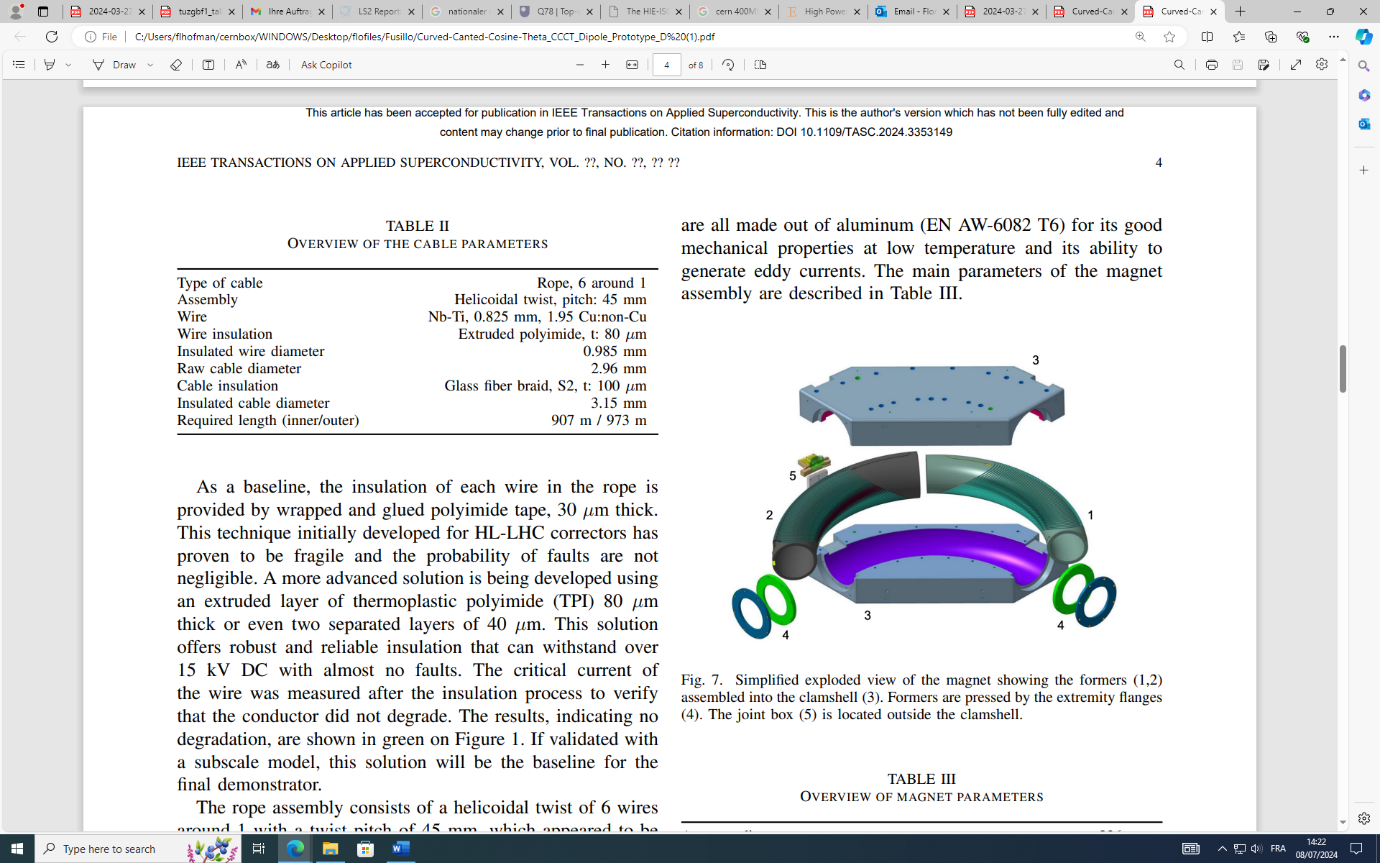
\includegraphics[width=2.95276in,height=1.97288in,alt={A screenshot of a computer Description automatically generated}]{images/media/image2.png}
\caption{\protect\phantomsection\label{_Ref225751343}{}\textbf{Figure
2.} Simplified exploded view of the magnet showing the inner (1) and
outer (2) formers, assembled into the clamshell (3). Formers are pressed
by the extremity flanges (4). The joint box (5) is located outside the
clamshell {[}3{]}}
\end{figure}

A sub-scale model was designed, to allow validation of the concept and
design (\hyperref[_Ref225747707]{Figure 3}). Following this, a
full-scale model was developed based on the insights gained. The
sub-scale has the same aperture and curvature radius, but it is spanning
only one-third of the full length, and thus achieves just a 30° bend
rather than the full 90°. Furthermore, the number of channels is reduced
to 2 turns instead of 65. In collaboration with the TE-MSC-SMT section,
responsible for conception assembly and testing of both configurations,
EN-MME group was involved in the mechanical design and in the
fabrication of the full-scale and sub-scale formers. This involved
material sourcing, development and testing of joining techniques, design
of clamping and tooling solutions, programming of multi-axis
manufacturing strategies, fabrication of the item and quality control.

The full context and motivation of the project, along with magnetic
simulation, optimisation, cable design, and initial test results, have
been comprehensively reported in literature {[}3{]} {[}4{]}. The scope
of this paper is to report on the mechanical design, as well as the
manufacturing process and its challenges.

\begin{longtable}[]{@{}
  >{\centering\arraybackslash}p{(\linewidth - 4\tabcolsep) * \real{0.1882}}
  >{\raggedright\arraybackslash}p{(\linewidth - 4\tabcolsep) * \real{0.0980}}
  >{\raggedright\arraybackslash}p{(\linewidth - 4\tabcolsep) * \real{0.0847}}@{}}
\caption{(a)
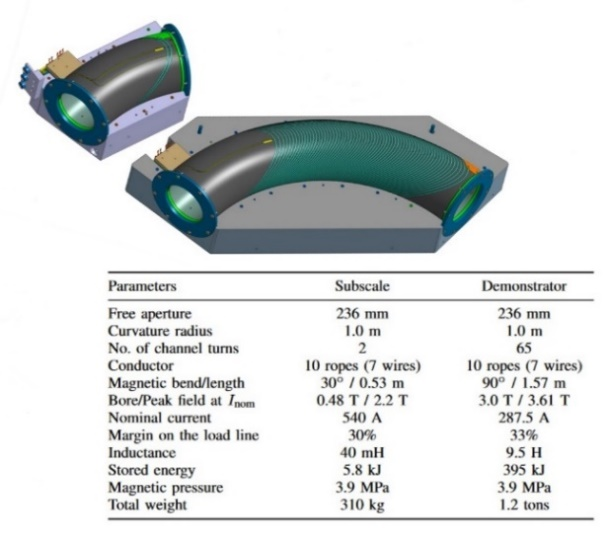
\includegraphics[width=2.70833in,height=1.45372in,alt={A diagram of a machine Description automatically generated with medium confidence}]{images/media/image3.jpeg}\\
(b)}\tabularnewline
\toprule\noalign{}
\begin{minipage}[b]{\linewidth}\centering
\textbf{Parameters}
\end{minipage} & \begin{minipage}[b]{\linewidth}\raggedright
\textbf{Sub-scale}
\end{minipage} & \begin{minipage}[b]{\linewidth}\raggedright
\textbf{Full-scale}
\end{minipage} \\
\midrule\noalign{}
\endfirsthead
\toprule\noalign{}
\begin{minipage}[b]{\linewidth}\centering
\textbf{Parameters}
\end{minipage} & \begin{minipage}[b]{\linewidth}\raggedright
\textbf{Sub-scale}
\end{minipage} & \begin{minipage}[b]{\linewidth}\raggedright
\textbf{Full-scale}
\end{minipage} \\
\midrule\noalign{}
\endhead
\bottomrule\noalign{}
\endlastfoot
Free aperture & 236 mm & 236 mm \\
Curvature radius & 1.0 m & 1.0 m \\
No. of channel turns & 2 & 65 \\
Magnetic bend/length & 30° / 0.53 m & 90° / 1.57 m \\
Total weight & 310 kg & 1.2 tons \\
\end{longtable}

\protect\phantomsection\label{_Ref225747707}{}\textbf{Figure 3.}
Graphical representation (a) and comparison table (b) of characteristics
of sub-scale Fusillo and full-scale demonstrator {[}3{]}

\section*{Description and function of the components}

The main components of the magnet can be seen in
\hyperref[_Ref225570545]{Figure 1}: two tapered formers - referred to as
inner and outer - are fit into each other, the clamshell and the flanges
contain the formers and provide insulation of the magnet; finally the
joint box makes the connection to the outside of the clamshell made from
extruded aluminium (EN AW-6082 T6) .

The tapered formers feature a machined groove on the outer surface,
which provides a channel to hold and guide the conductor. Ten rope
cables of seven insulated wires each are wound on the inner former, over
which the outer former is then slid. This encasing is facilitated by the
tapered design: one end features a 10 mm smaller diameter than the other
end.

Sufficient space for the insertion after winding is provided. The
conical shape is mirrored on inner and outer surfaces of the formers,
resulting in a tapered coil. Exiting the inner former with a layer jump
(Figure 4), the winding continues in the outer former. This assembly is
then enclosed in a clamshell and connected with flanges at the
extremities to hold against generated magnetic forces, bending the
assembly. The fabrication procedure of the formers, the most complex
component, is explained in the following section.

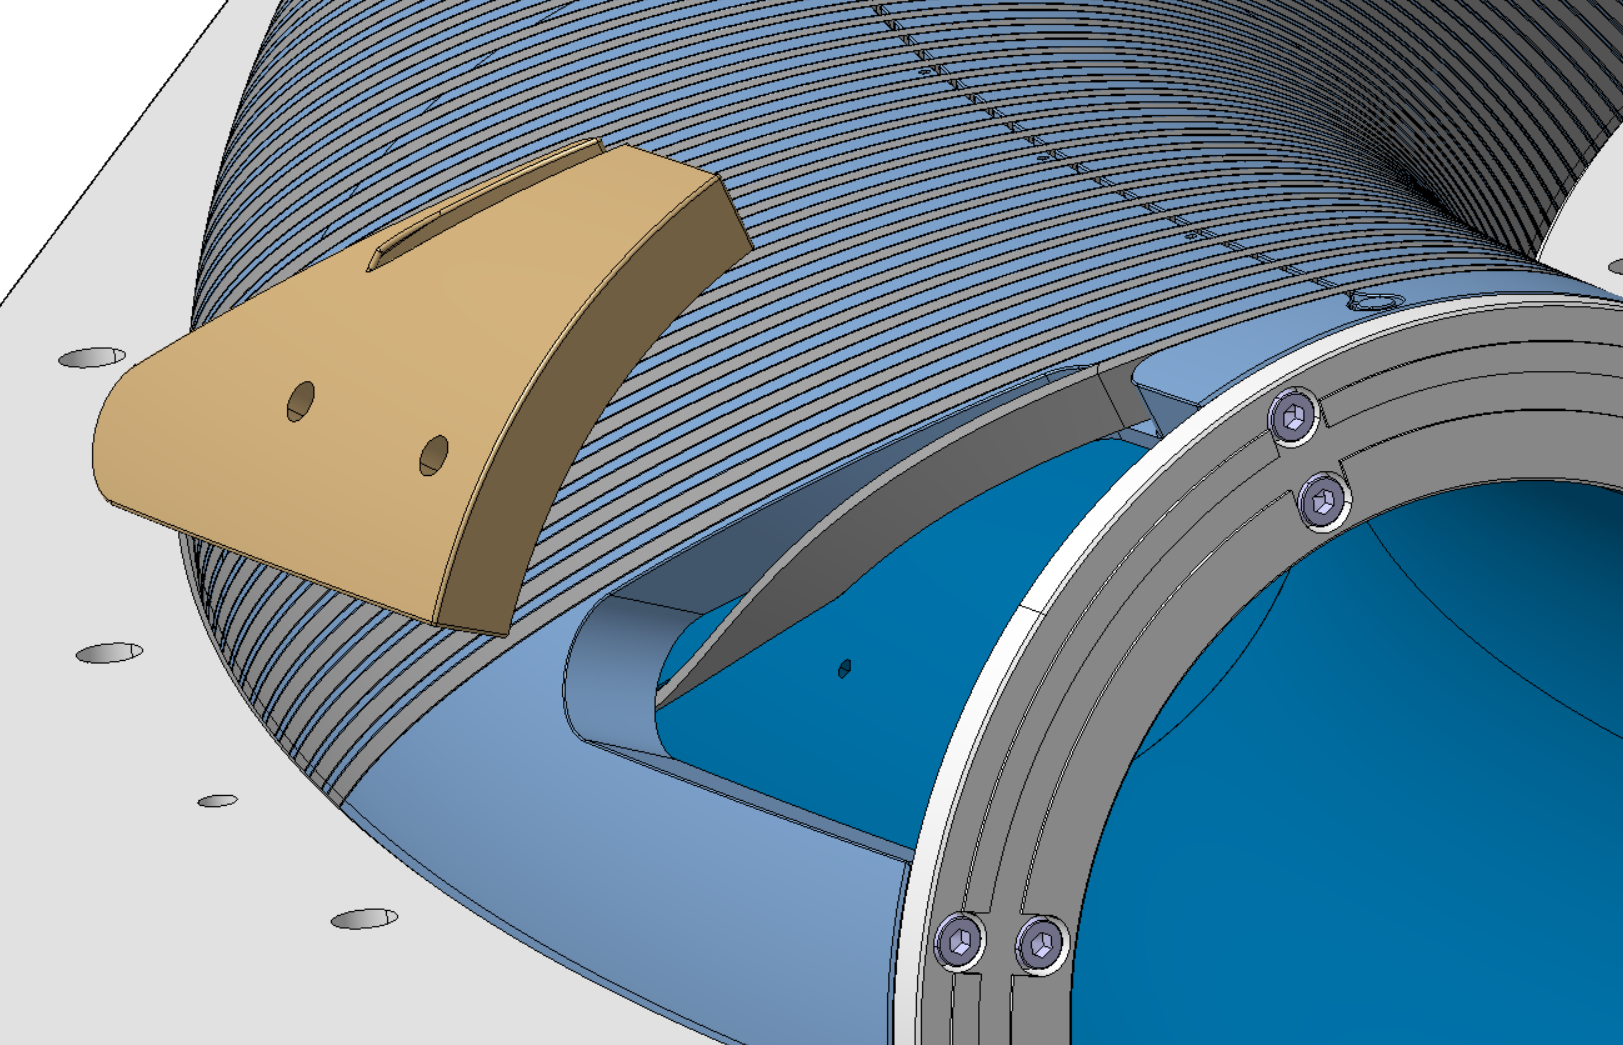
\includegraphics[width=3.38819in,height=2.18125in]{images/media/image4.png}

\textbf{Figure} \textbf{4.} Representation of the inner former (dark
blue), outer former (light blue), and coil (dark grey), with the layer
jump (brown) depicted in an exploded view.

Further assembly steps by the TE-MSC-SMT section included the precise
positioning of cables before joining the inner and outer formers and
resin impregnation after closing the clamshell. Intensive testing of the
sub-scale prototype was performed to demonstrate the practicality of the
design before proceeding with the full-scale demonstrator

\section*{Manufacturing Process sub-scale prototype}

EN-MME engaged in the production of the inner and outer formers for the
sub-scale Fusillo magnets. The machining sequences consisted of four
steps:

\begin{enumerate}
\def\labelenumi{\arabic{enumi}.}
\item
  Horizontal setup on V-clamps for roughing and finishing interior and
  end surfaces (\hyperref[_Ref225572043]{Figure 5}).
\item
  Vertical setup with additional blocks fixed in the chuck, secured
  internally using a threaded rod for roughing and finishing the
  exterior envelope (\hyperref[_Ref225571883]{Figure 7}).
\item
  Horizontal setup on additional blocks to allow machining of the outer
  surface, including cable channels and features such as the connection
  box\\
  (\hyperref[_Ref225571922]{Figure 6}).
\item
  Horizontal setup rotated 180° from setup 3.
\end{enumerate}

A key manufacturing challenge in roughing the formers from pre-cored
billets, as encountered for monobloc ISOLDE cavities {[}5{]}, was the
use of very long tool extensions (over 600 mm for interior machining),
which were prone to chatter.

\begin{figure}
\centering
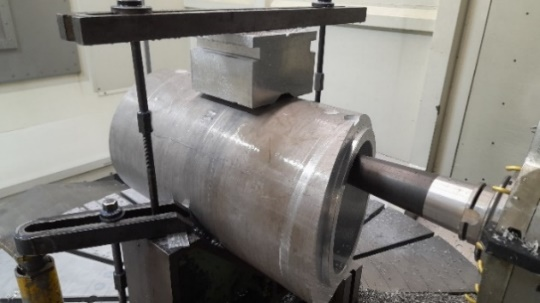
\includegraphics[width=2.44024in,height=1.32778in]{images/media/image5.jpeg}
\caption{\protect\phantomsection\label{_Ref225572043}{}\textbf{Figure
5.} First Setup for interior roughing and milling with Long toolholder
attached.}
\end{figure}

To ensure positioning accuracy over the entire process, two reference
blocks have been manufactured and adapted to fit into the apertures of
the formers, azimuthal positioning being secured with standard dowel
pins (\hyperref[_Ref225571922]{Figure 6}). These blocks, featuring
milled pockets, provide well-defined reference geometries to execute
control and measurement cycles with the machines integrated 3D measuring
probe. They also serve as fixture tooling
(\hyperref[_Ref225571922]{Figure 6}).

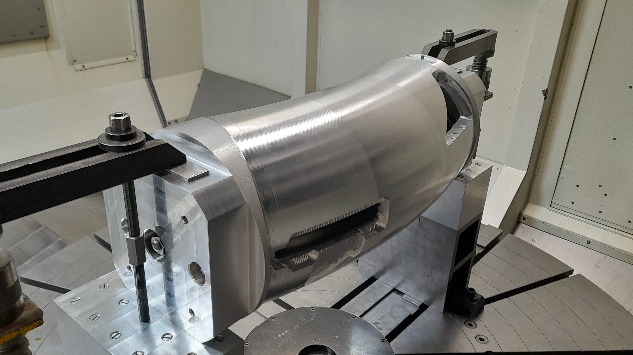
\includegraphics[width=2.88751in,height=1.55556in,alt={A close-up of a machine Description automatically generated}]{images/media/image6.jpeg}

\protect\phantomsection\label{_Ref225571922}{}\emph{\textbf{Figure 6.}
Horizontal position.} \emph{reference block can be seen on the left part
of the item.}

The outer formers of the sub-scale Fusillo were manufactured on a 5-axis
machine with a rotating table. This capability was extensively used
during envelope finishing: after a highly dynamic roughing cycle removed
most of the material, leaving a 2 mm allowance, a 20 mm carbide
ball-nose mill performed the semi-finishing and finish machining in a
single continuous spiral, with simultaneous 5-axis motion
(\hyperref[_Ref225571883]{Figure 7}).

\begin{figure}
\centering
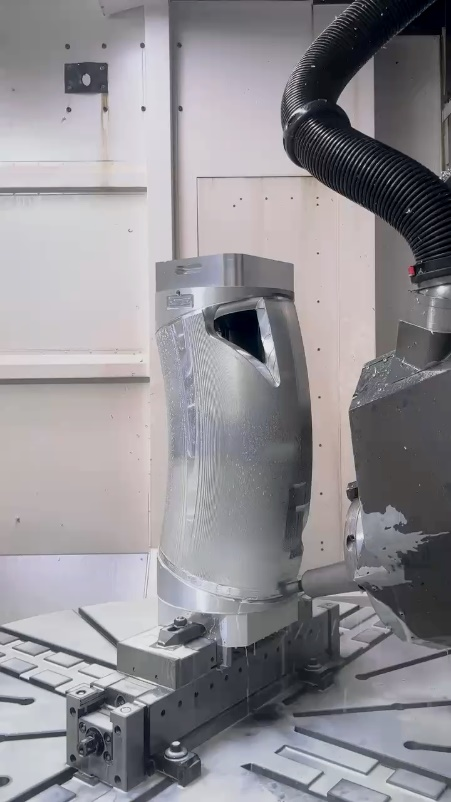
\includegraphics[width=2.03571in,height=3.61916in]{images/media/image7.jpeg}
\caption{\protect\phantomsection\label{_Ref225571883}{}\textbf{Figure
7.} Vertical positioning of the component with positioning blocks on top
and bottom during exterior finishing}
\end{figure}

\section*{Manufacturing of full-scale demonstrator}

The full-scale demonstrator was designed using a segmented approach,
with spanning angles of 35°, 30°, and 25° for both the outer and inner
formers.

\begin{figure}
\centering
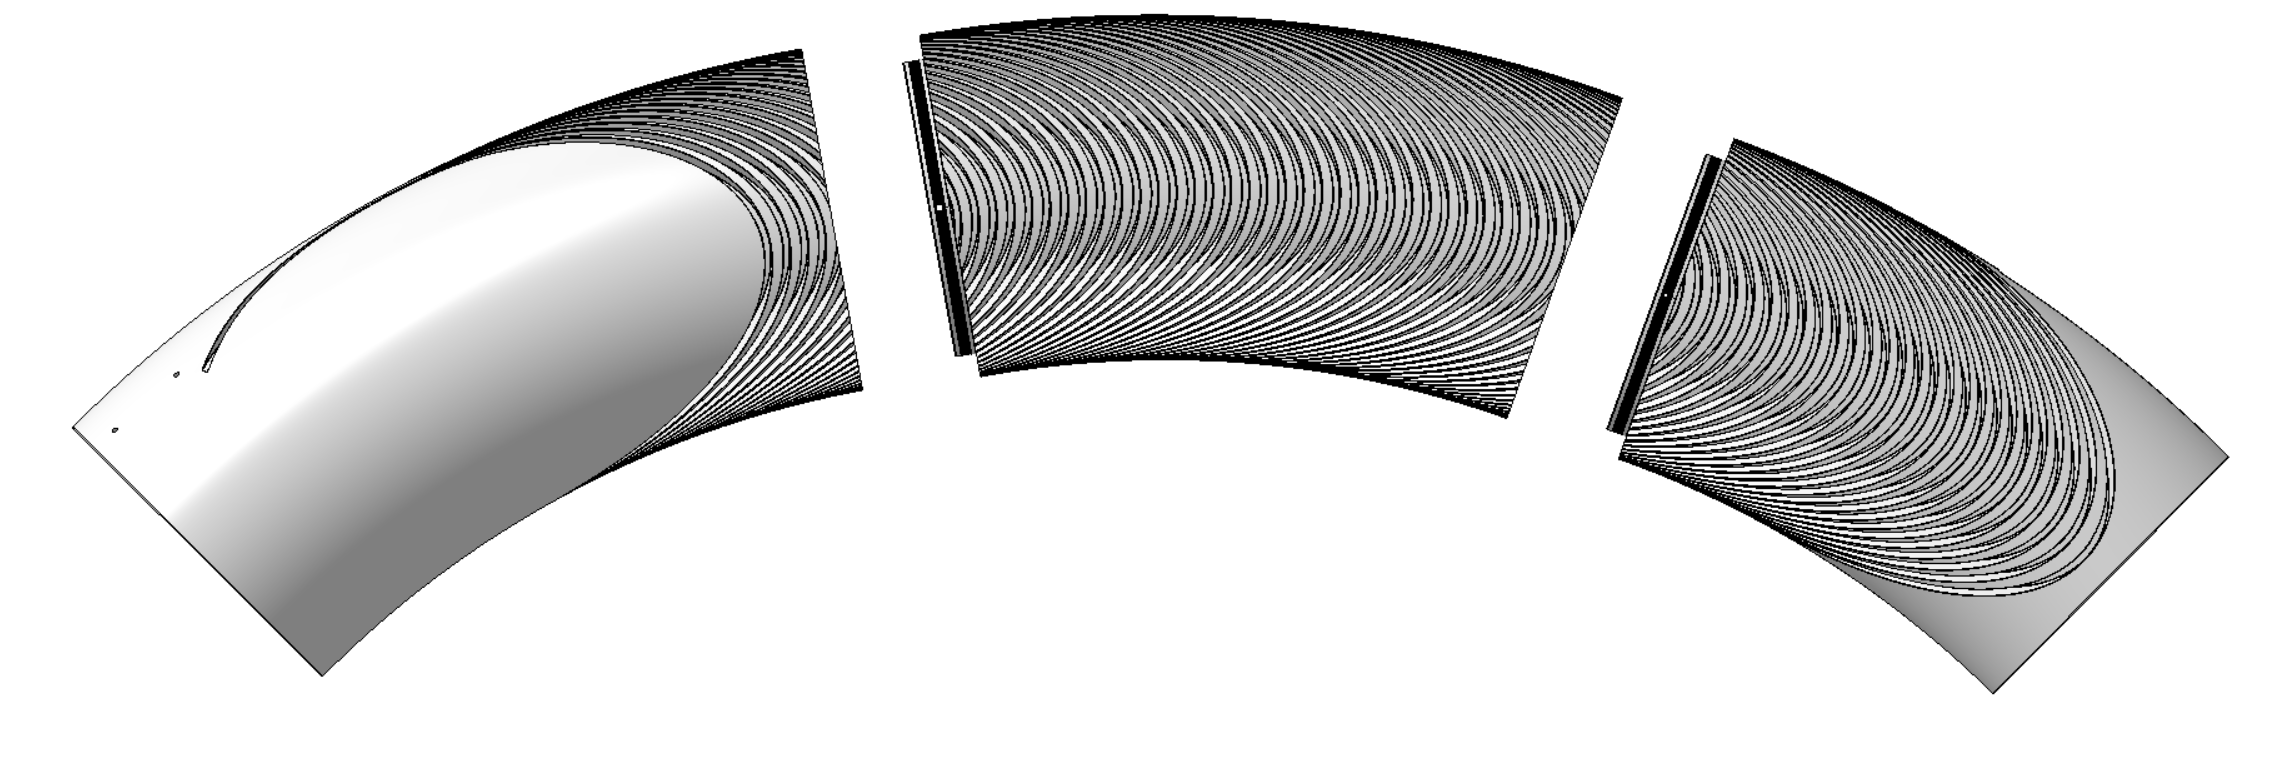
\includegraphics[width=3.14961in,height=1.01272in]{images/media/image8.png}
\caption{\textbf{Figure 8.} Representation of the full-scale inner
former made of 3 segments.}
\end{figure}

The adopted machining sequence involved machining the internal surfaces
of each segment, as first step. Once completed, all segments were
assembled, after which the external surfaces were machined to achieve
the final winding geometry. Compared to the sub-scale prototypes, these
setups were adapted because finishing the 90° former in a vertical setup
proved impractical due to milling machine angle limitations.
Consequently, the machining of the external surfaces was carried out
using a horizontal setup.

For the assembly, positioning was ensured by machining two cylindrical
contact surfaces on the sides of each segment, to achieve concentric
alignment, along with a dowel pin to control azimuthal positioning.
(Initial trials employed thermal fitting using liquid nitrogen, based on
the principle of shrink-fitting; however, this approach did not provide
sufficient resistance to separation). The adopted solution involved
injecting Stycast epoxy resin into orbital grooves located at the
interfaces between segments. Once cured, the epoxy acts as five
circumferential (orbital) pins, thereby providing the required
mechanical retention and positional stability
(\hyperref[_Ref225755796]{Figure 9}).

\begin{figure}
\centering
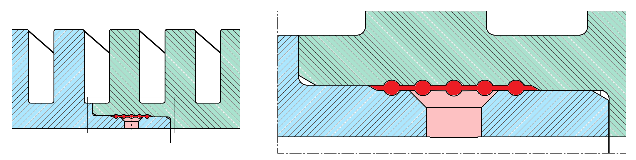
\includegraphics[width=2.88819in,height=0.725in]{images/media/image9.png}
\caption{\protect\phantomsection\label{_Ref225755796}{}\textbf{Figure
9.} Illustration of the assembly technique, showing the machined grooves
and holes for Epoxy Resin injection, cross section view.}
\end{figure}

LOCTITE STYCAST EE 4215/HD 3561 was selected as the injection resin due
to its favourable mechanical and electrical properties. Its Shore D
hardness of 83 provides the necessary stability for precise alignment
within the machined channels, acting as an effective mechanical lock
once cured. In conclusion this process offered favourable parameters
regarding separation resistance, as confirmed by initial test samples. A
finite element simulation was performed (Figure 10) assuming a
conservative friction coefficient (µ = 0.25), along with no adhesive
bonding between the resin and aluminium. Only negligible stress and
separation of the two formers have been calculated under a tensile load
of 6kN.

\begin{figure}
\centering
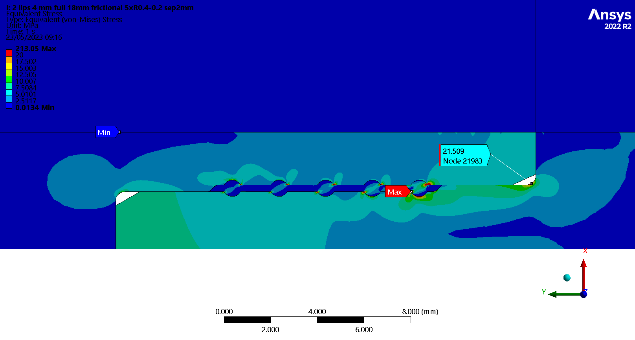
\includegraphics[width=2.88819in,height=1.54444in]{images/media/image10.png}
\caption{\textbf{Figure 10.} FEM simulation depicting the distribution
of tensile load applied to the assembly, plotting stress under applied
forces.}
\end{figure}

The joint was validated on a full-scale cylindrical mock-up undergoing a
test to failure. The channels for the epoxy were machined using a
standard slot-milling tool with a rounded geometry (r = 1 mm) and a
depth of 0.3 mm, resulting in a cross-sectional area larger than in the
simulation, where R0.4 x 0.2 was assumed. A tensile pulling test on the
mock-up of the joint assembly showed structural integrity under loads
exceeding 40 kN with zero plastic deformation and an elastic separation
of less than 5 µm. This mechanical stability is crucial not only for
subsequent handling of the assembly but also for withstanding the
bending forces induced by the magnetic field. Complete separation (i.e.
failure) occurred at 67 kN (\hyperref[_Ref225756340]{Figure 11}).

\begin{figure}
\centering
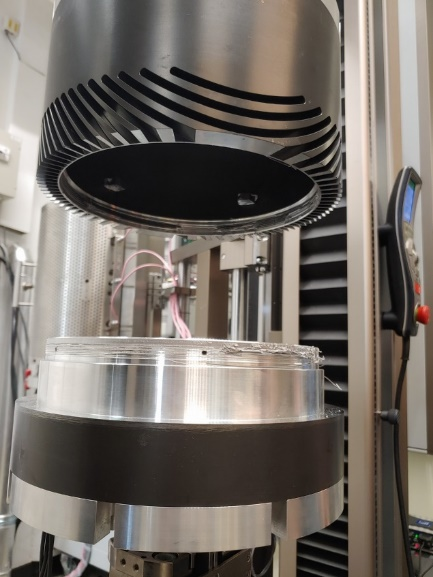
\includegraphics[width=1.9685in,height=2.62451in]{images/media/image11.jpeg}
\caption{\protect\phantomsection\label{_Ref225756340}{}\textbf{Figure
11.} Destructive testing of the full-scale cylindrical mock-up to
complete separation.}
\end{figure}

The resin was injected into opposing holes from the interior of the
assembly using a 3D-printed applicator (\hyperref[_Ref225755994]{Figure
12}), while two additional holes allowed air to escape from the
interior.

\begin{figure}
\centering
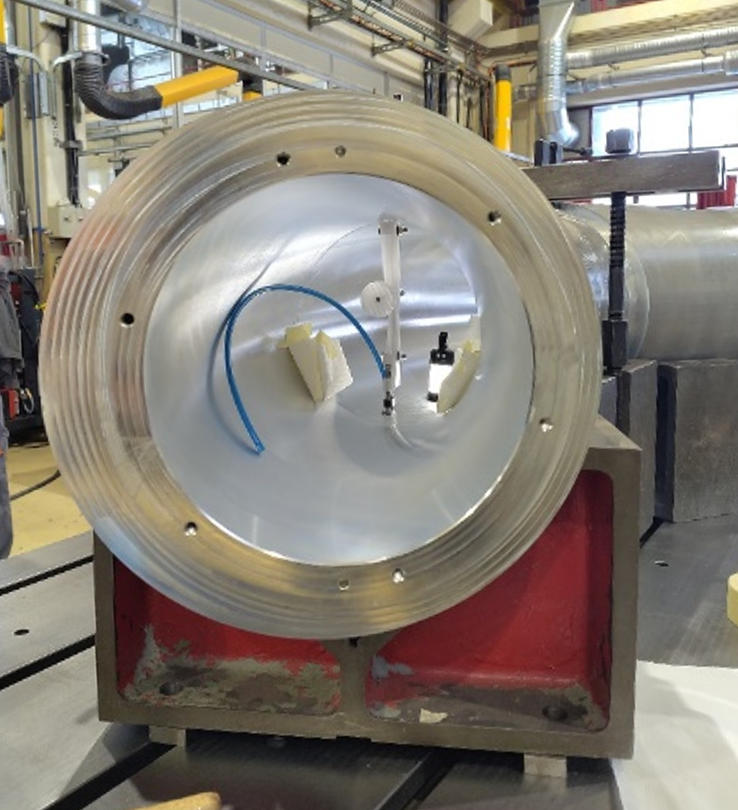
\includegraphics[width=1.9685in,height=2.16067in]{images/media/image12.png}
\caption{\protect\phantomsection\label{_Ref225755994}{}\textbf{Figure
12.} Assembly of the full-scale former with the 3D printed applicator
visible inside the part.}
\end{figure}

\section*{Machining of the outer surface and channels}

After assembly into the full 90° former, machining of the outer surfaces
and channels was carried out on a Waldrich-Coburg Taurus 30 in three
successive stages. The process began with the top side, where roughing
was performed using a high-torque HSK-A100 machining head, followed by
semi-finishing with an HSK-A63 high-speed head. Equivalent operations
were then carried out on the bottom side, where final surface finishing,
as well as the milling of grooves and features, was completed. In the
final stage, the remaining grooves and features on the top side were
machined, thereby completing the component.
(\hyperref[_Ref225767419]{Figure 14}).

\begin{figure}
\centering
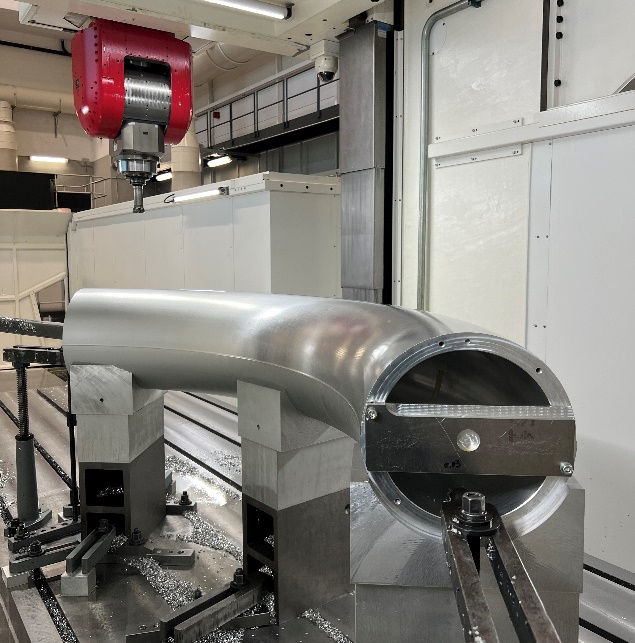
\includegraphics[width=2.88976in,height=2.9252in]{images/media/image13.jpeg}
\caption{\protect\phantomsection\label{_Ref225761556}{}\textbf{Figure
13.} Machining of the Channels and finishing of the top surface.}
\end{figure}

During the roughing step, probing measurements were performed on
reference surfaces machined on the exterior of the formers in order to
align the component with the metrology-derived reference frame, which
had previously been established through a best-fit alignment of the
interior surfaces. Additionally, auxiliary metal plates featuring
machined pockets were attached to the faces and served as reference
surfaces throughout the machining sequence
(\hyperref[_Ref225761556]{Figure 13}).

For the subsequent machining steps, a custom fixture was manufactured in
situ, without dismantling the part, to ensure stable clamping and
precise positioning within the machine. Clamping force was applied at
three defined key points corresponding to the support locations to
minimize vibration as effectively as possible during machining. This
fixture was re-machined between the semi-finishing and finishing stages
to accommodate the change in dimensions.

For the finishing of the channels, a custom-made end mill was employed.
This tool was specifically designed to ensure smooth, rounded
transitions at both the bottom and shoulder of the channels, featuring a
radius of r = 0.25 mm at both the tip and shank, thus adhering to the
specified tolerances of the geometry in one pass.

\begin{figure}
\centering
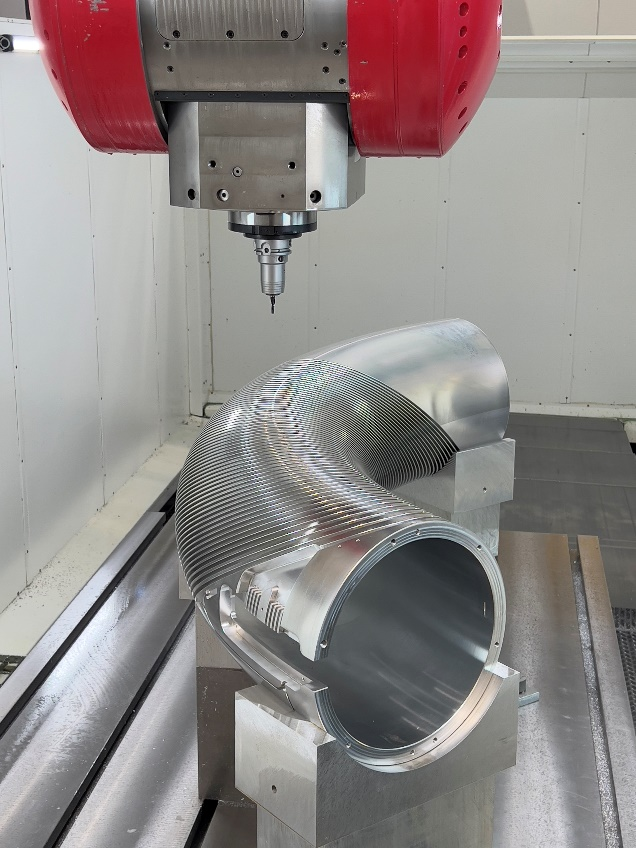
\includegraphics[width=2.88819in,height=3.30833in]{images/media/image14.jpeg}
\caption{\protect\phantomsection\label{_Ref225767419}{}\textbf{Figure
14.} Former after all machining operations were performed.}
\end{figure}

\section*{Toolpath definition}

Due to the conical geometry of the formers, the channel layout does not
exhibit repetitive patterns. Given the large number of geometrical
features to be manufactured, a programmatic approach was adopted for
toolpath definition (\hyperref[_Ref225761556]{Figure 13}). This approach
also provided an extended level of control over the toolpaths, exceeding
the capabilities of conventional CAM software. The approach also enabled
the generation of all required toolpaths from a single procedure,
including 5-axis pilot drilling, roughing and finishing of the grooves,
as well as transitional toolpaths to ensure smooth connections between
grooves machined from opposite sides. To prevent overtravel of the
machine's rotary C-axis, the toolpaths were segmented at predefined
angular intervals.

The toolpath definition was derived from data extracted directly from
the CAD model, including the centreline of the channels and the
corresponding surface normal vectors, using the open-source software
FreeCAD, which supports advanced macro programming. These data were then
used to generate toolpaths through matrix-based computations, requiring
only minimal positional adjustments of the tool within the groove
geometry (\hyperref[_Ref225772091]{Figure 15}). The resulting toolpaths
were subsequently imported into the commercial CAM software WorkNC by
encoding them in the appropriate format, enabling them to be recognized
as native toolpaths. This allowed the custom-generated toolpaths to
benefit from WorkNC's built-in capabilities, such as collision detection
and post-processing, while maintaining full control over the toolpath
geometry. This hybrid approach effectively combined the flexibility of
custom-defined toolpaths with the robustness and usability of advanced
CAM software.

\begin{figure}
\centering
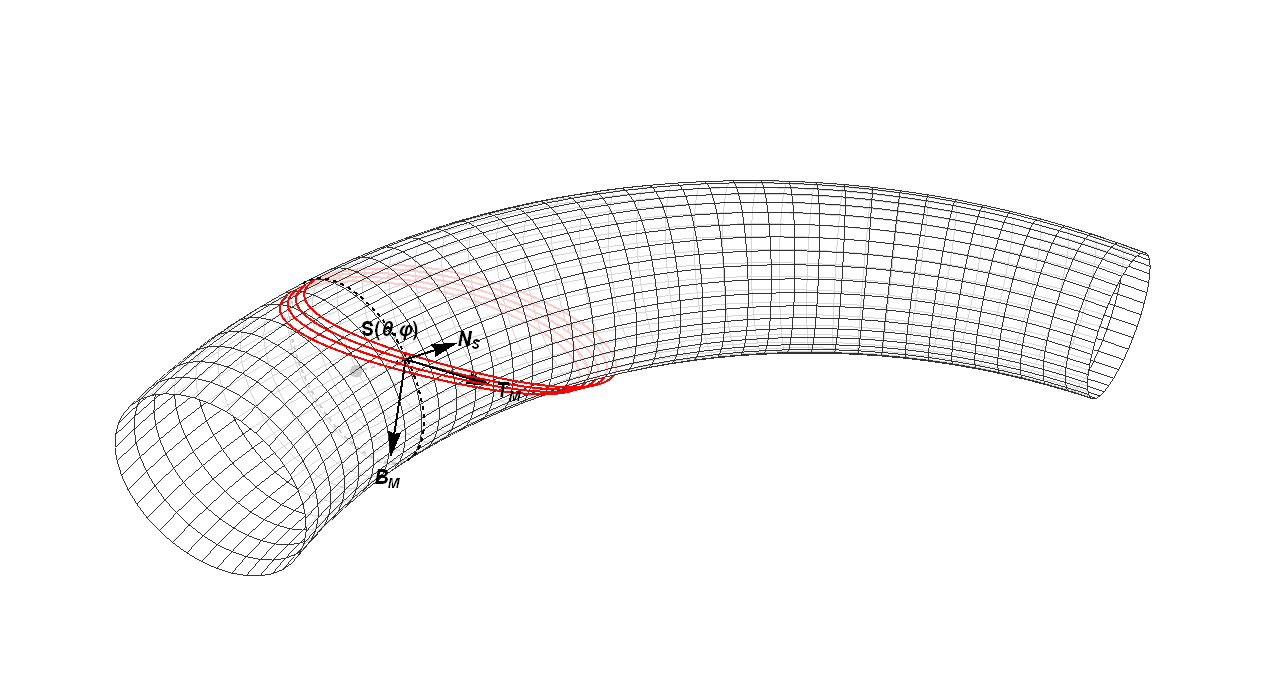
\includegraphics[width=2.96351in,height=2.11409in]{images/media/image15.png}
\caption{\protect\phantomsection\label{_Ref225772091}{}\textbf{Figure
15.} Visual representation of the toolpath at a given point,
illustrating the normal, tangential, and binormal directions defining
the local toolpath coordinate frame.}
\end{figure}

\section*{Conclusion}

The manufacturing and assembly of the Fusillo curved canted cosine theta
(CCCT) dipole magnet represent a significant achievement in precision
engineering under complex geometric and mechanical constraints. By
combining a design-for-manufacturing approach, an innovative joining
technique, tailored clamping solutions, advanced 5-axis programming
techniques, and metrology-driven feedback loops, it was possible to
produce both sub-scale and full-scale prototypes that meet the
requirements for superconducting magnet formers.

This experience not only deepens our understanding of multi-stage
manufacturing but also lays the groundwork for future complex
large-scale components manufacturing. The Fusillo project thus stands as
a template of the collaborative and interdisciplinary approach applied
at CERN to transform a challenging theoretical design into a
manufacturable and functional physical prototype.

\section*{References}

{[}1{]} G. A. Kirby \emph{et al}., ``Hi-Lumi LHC twin-aperture orbit
correctors magnet system optimisation,'' \emph{IEEE Transactions on
Applied Superconductivity}, vol. 27, no. 4, Art. no. 4002805, Jun. 2017.
doi: 10.1109/TASC.2016.2633424

{[}2{]} G. A. Kirby \emph{et al}., ``Superconducting curved
canted-cosine-theta (CCT) for the HIE-ISOLDE recoil separator ring at
CERN,'' \emph{IEEE Transactions on Applied Superconductivity}, vol. 32,
no. 6, Sep. 2022. doi: 10.1109/TASC.2022.3158332

{[}3{]} A. Haziot \emph{et al}., ``Curved canted-cosine-theta (CCCT)
dipole prototype development at CERN,'' \emph{IEEE Transactions on
Applied Superconductivity}, vol. 34, no. 2, Aug. 2024. doi:
10.1109/TASC.2024.3353149

{[}4{]} M. Woźniak \emph{et al}., ``Transient behavior of the second
Fusillo subscale curved CCT magnet,'' \emph{IEEE Transactions on Applied
Superconductivity}, Jan. 2025. doi: 10.1109/TASC.2025.3540828

{[}5{]} S. Delsolaro \emph{et al}., ``Seamless quarter-wave resonators
for HIE-ISOLDE.'' Available:
https://cds.cern.ch/record/2669959/files/tu1a05.pdf

\end{document}
